\documentclass{beamer}
\usepackage{pgfplots}
\usepackage{filecontents}
\usepackage{tikz}
\usepackage{etex}
\usepackage{verbatim}
\pgfplotsset{compat=1.8}
\usepackage{pgfplotstable}
\usepackage{tikz-qtree}
\usepackage{tikz-dependency}
\tikzstyle{vertex}=[draw,fill=black!15,circle,minimum size=10pt,inner sep=1pt]

\begin{document}
\begin{frame}[fragile]{A* on a Min-Heap}
\begin{figure} 
  \centering
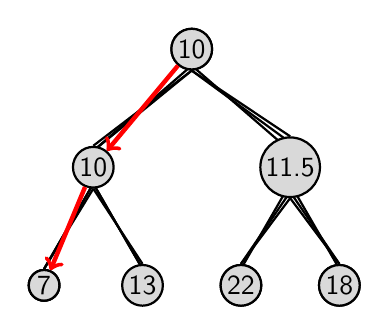
\begin{tikzpicture}[font=\sffamily,thick,level/.style={sibling distance=25mm/#1}]
  \onslide<1>{
    \node[vertex] {0}
    child {
      node[vertex] {1}
      child {
        node[vertex] {3}
      }
      child{
        node[vertex] {5}
      }
    }
    child {
      node[vertex] {2}
      child { node[vertex] {6} }
      child { node[vertex] {4} }
    };
  }
  \onslide<2>{
    \node[vertex] {10}
    child {
      node[vertex] {9}
      child {
        node[vertex] {4}
      }
      child{
        node[vertex] {8}
      }
    }
    child {
      node[vertex] {9.5}
      child { node[vertex] {16} }
      child { node[vertex] {14} }
    };
  }
  \onslide<3->{
    \node[vertex] (a) {10}
    child {
      node[vertex] (b) {10}
      child {
        node[vertex] (c) {7}
      }
      child{
        node[vertex] {13}
      }
    }
    child {
      node[vertex] {11.5}
      child { node[vertex] {22} }
      child { node[vertex] {18} }
    };
  }
  \onslide<4>{
    \path[draw, red, ultra thick, ->] (a) -- (b);
    \path[draw, red, ultra thick, ->] (b) -- (c);
  }

\end{tikzpicture}
\end{figure}
\begin{center}
    \only<1>{
    $Cost()$
  }
  \only<2>{
    $Heuristic()$
  }
  \only<3>{
    $Cost()+Heuristic()$
  }
  \only<4>{
    $\min Cost()+Heuristic()$
  }
\end{center}
\end{frame}

\begin{frame}[fragile]{A* on a Max-Heap (of Gumbels)}
\begin{figure} 
  \centering
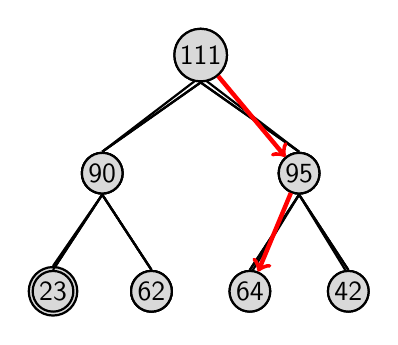
\begin{tikzpicture}[font=\sffamily,thick,level/.style={sibling distance=25mm/#1}]
  \onslide<1>{
    \node[vertex] {100}
    child {
      node[vertex] {70}
      child {
        node[vertex] {33}
      }
      child{
        node[vertex] {50}
      }
    }
    child {
      node[vertex] {82}
      child { node[vertex] {63} }
      child { node[vertex] {41} }
    };
  }
  \onslide<2>{
    \node[vertex] {11}
    child {
      node[vertex] {20}
      child {
        node[vertex] {-10}
      }
      child{
        node[vertex] {12}
      }
    }
    child {
      node[vertex] {13}
      child { node[vertex] {1} }
      child { node[vertex] {1} }
    };
  }
  \onslide<3->{
    \node[vertex] (a) {111}
    child {
      node[vertex] {90}
      child {
        node[vertex] {23}
      }
      child{
        node[vertex] {62}
      }
    }
    child {
      node[vertex] (b) {95}
      child { node[vertex] (c) {64} }
      child { node[vertex] {42} }
    };
  }
  \onslide<4>{
    \path[draw, red, ultra thick, ->] (a) -- (b);
    \path[draw, red, ultra thick, ->] (b) -- (c);
  }

\end{tikzpicture}
\end{figure}
\begin{center}
  \only<1>{
    $Utility()$\\
    (Think Gumbel Maxes, $G_i$) \\
    Heap on $G$ values, each node is $(G_i,X_i)$ \\
  }
  \only<2>{
    $Heuristic()$\\
    (Think $o(X_i)$)
  }
  \only<3>{
    $Cost()+Heuristic()$\\
    (Think $G_i + o(X_i)$)
  }
  \only<4>{
    $\max Utility()+Heuristic()$ \\
  }
  \only<5>{
    Not as simple, as we only know bounds of $o(X)$
  }
\end{center}
\end{frame}

\end{document}
